\documentclass{bmd2016p}
\usepackage{epstopdf}

\begin{document}

\begin{center}
\fontsize{14}{20}{\bf Buckling and dynamic collapse of the bicycle wheel}
\end{center}

%%%%%%%%%%%%%%%% authors %%%%%%%%%%%%%%%
\begin{center}
\normalsize{\bf{Matthew Ford$^{*}$, Jim M. Papadopoulos$^\#$, 
            Oluwaseyi Balogun$^\dag$}}
\end{center} 

\begin{center}
\begin{tabular}{c}
$^*$ Department of Mechanical Engineering\\
Northwestern University\\
2145 Sheridan Road, Evanston, IL 60208, USA\\
e-mail: mford@u.northwestern.edu\\[2.5ex]

$^\#$ Department of Mechanical and Industrial Engineering\\
Northeastern University\\
360 Huntington Ave., Boston, MA 02115, USA\\
e-mail: j.papadopoulos@neu.edu\\[2.5ex]

$^\dag$ Department of Civil Engineering\\
Northwestern University\\
2145 Sheridan Road, Evanston, IL 60208, USA\\
e-mail: o-balogun@northwestern.edu\\
\end{tabular}
\end{center}

\section*{ABSTRACT}

...

\begin{keywords}
bicycle wheel, 
buckling, 
bifurcation.
\end{keywords}





\section{INTRODUCTION}

The bicycle wheel is a prestressed structure and is susceptible to buckling under internal forces. As the spokes are tightened uniformly, the rim deforms radially to accommodate the spoke strain. At a critical tension, the system reaches a bifurcation point and the rim buckles out of its initial plane. The post-buckling configuration is generally stable and the original shape of the wheel can be recovered by reducing the tension. Buckling can also be triggered by external forces in an otherwise stable wheel leading to a release of strain energy. This is an unstable process which generally leads to catastrophic failure.

Despite its implications for wheel strength, the buckling problem has never received a rigorous treatment to our knowledge. Jobst Brandt alludes to buckling in his practical manual for wheelbuilders~\cite{Brandt1993c}:

\begin{quotation}
\noindent``If the wheel becomes untrue in two large waves during stress relieving, the maximum, safe tension has been exceeded. Approach this tension carefully to avoid major rim distortions. When the wheel loses alignment from stress relieving, loosen all spokes a half turn before retruing the wheel.''
\end{quotation}

He did not discuss the problem further, but suggested that wheel failure commonly occurs due to a loss of lateral stability caused by spoke buckling. Pippard and Francis~\cite{Pippard1932d} derived a model for lateral stiffness based on the elastic foundation model, but did not discuss stability and neglected any effects of spoke tension.

Flexural-torsional buckling of rings can be treated as a special case of buckling of arches, where the included angle is allowed to go to $2\pi$. Timoshenko and Gere~\cite{Timoshenko1961a} gave a formula for the critical load for a ring with doubly-symmetric cross-section subjected to radial loads. The theory of flexural-torsional buckling of monosymmetric arches (bicycle rims have only one plane of symmetry) was broadly formalized by Trahair and Papangelis~\cite{Trahair1987b} using the virtual work approach to derive the equilibrium and stability equations. Their theory has been extended to treat arches restrained by continuous~\cite{Pi2002b} or discrete~\cite{Bradford2002d} elastic supports and elastic end restraints~\cite{Guo2014b}.

The problem of the prestressed bicycle wheel is unique for a number of reasons. First, the buckling load is internal to the structure. Second, the spokes act both as elastic restraints resisting buckling and as prestressing elements causing buckling. Third, the lateral, radial, and torsional restraining actions of the spokes are coupled---i.e. lateral deflection at a spoke may produce lateral, radial, and torsional reactions. These considerations extend to other structural systems. Large observation wheels such as the London Eye~\cite{Mann2001a} and the Singapore Flyer~\cite{Allsop2009a} resemble large bicycle wheels and achieve lateral stability due to the bracing angle of prestressed cables, and must be designed against flexural-torsional buckling.

Here we derive a general theory for buckling of a spoked bicycle wheel under self-tension and investigate several special cases. Furthermore, we analyze large deformation post-buckling behavior and show how local buckling of individual spokes can lead to collapse of an otherwise sub-critical wheel.




\section{DEFORMATION OF THE WHEEL}
A typical bicycle wheel (Fig. \ref{fig:schematic} consists of a slender rim connected to a hub by means of a system of very slender metal spokes. The spokes are usually threaded at the rim side into spoke nipples which are inserted through the rim from the outside. The spokes are kept under tension by the rim. Without pretension, the spokes would immediately buckle under a very small load due to their high aspect ratio.

\begin{figure}[!h]
\centering
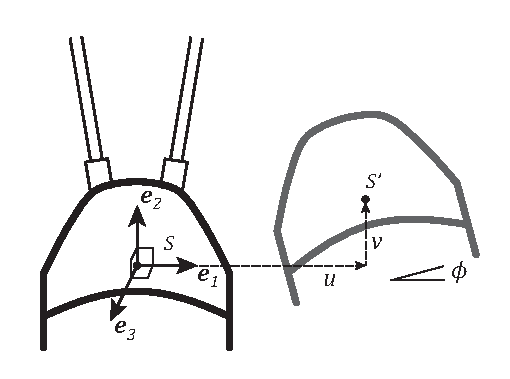
\includegraphics[scale=1.0]{figures/bmd_figures-06.eps}
\caption{caption}
\label{fig:schematic}
\end{figure}

To hold the spokes under tension, the rim must be under compression. An accurate approximation\footnote{95\% accurate for 6 spokes, $\alpha=10^{\circ}$, $\beta=10^{\circ}$. Increasing the number of spokes only improves the estimate.} was given by Sharp~\cite{Sharp1977a} by considering a force balance on the top (or bottom) half of the rim.
	\begin{equation}\label{eq:TN}
	N_r = \frac{n_sT}{2\pi}
	\end{equation}
The spokes act like guy-wires, both supporting the rim radially and stabilizing the rim laterally. However, if the spoke tension exceeds a critical value $T_c$, the compression in the rim causes the wheel to buckle laterally, bending and twisting out of its initial plane, as shown in Fig. \ref{fig:schematic} (c).


\subsection{Rim equations}

The rim is modeled as an initially circular beam with a constant cross-section. For simplicity we will assume that the shear center and centroid of the cross-section coincide. Except for warping deformation, plane cross-sections remain planar and shear flexibility of the cross-section is neglected. Furthermore, we assume that the rim radius is much larger than the height of the rim profile.

\begin{figure}[!ht]
\centering
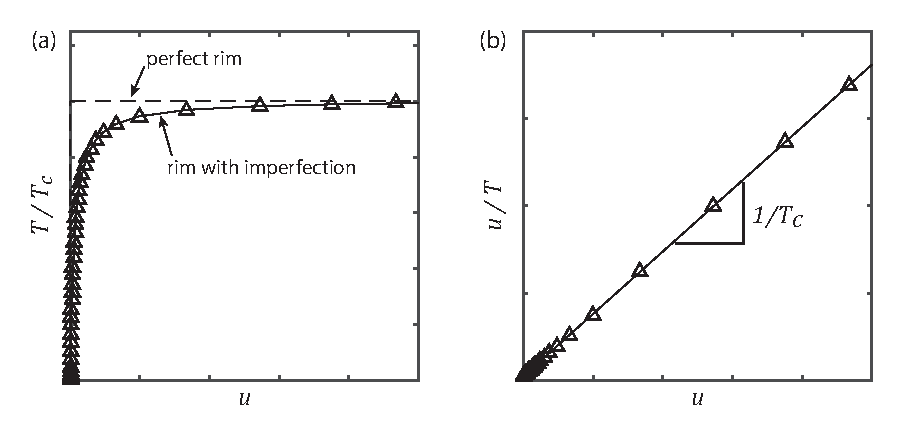
\includegraphics[scale=1.0]{figures/bmd_figures-07.eps}
\caption{Deformation of a rim cross-section. The shear center $S\rightarrow S'$ translates by the vector $\bm{u} = u\hat{\bm{e}}_1 + v\hat{\bm{e}}_2 + w\hat{\bm{e}}_3$ and rotates through an angle $\phi$.}
\label{fig:def}
\end{figure}

The in-plane curvature $\kappa_1$ is assumed to remain constant during flexural-torsional buckling. The in-plane curvature, out-of-plane curvature and twist rate are
	\begin{equation}\label{eq:k1}
	\kappa_1 = 1/R
	\end{equation}
	\begin{equation}\label{eq:k2}
	\kappa_2 = u'' - \frac{\phi}{R}
	\end{equation}
	\begin{equation}\label{eq:k3}
	\kappa_3 = \phi' + \frac{1}{R} u'
	\end{equation}
The symbol $()'$ indicates a derivative with respect to $s$. It can easily be verified that Equations \ref{eq:k2} and \ref{eq:k3} simplify to the standard equations for straight beams in the limit $R\rightarrow \infty$. The curvature and twist rate produce a bending moment and twisting moment equal to
	\begin{equation}\label{eq:M2}
	M_2 = EI_{11} \kappa_2
	\end{equation}
	\begin{equation}\label{eq:M3}
	M_3 = GJ \kappa_3 + EI_w \kappa_3''
	\end{equation}
The total strain energy is decomposed into lateral bending, uniform torsion, and warping terms which are related to the curvatures.
	\begin{equation}\label{eq:Urim}
	U_{rim} = \int_0^{2\pi} \left( \frac{1}{2} EI_{22} \kappa_2^2 + \frac{1}{2} GJ \kappa_3^2 + \frac{1}{2} EI_w (\kappa_3')^2 \right)\, ds
	\end{equation}
After buckling, a differential line segment $ds$ deforms to $dS$. The apparent shortening of the line segment along the $s$ direction is then
	\begin{equation}\label{eq:ds}
	ds - dS = ds - \sqrt{ds^2 + \left(\frac{du}{ds}ds\right)^2} \approx \frac{1}{2} (u')^2 \, ds
	\end{equation}
The axial compressive force in the rim moves through this differential displacement, performing virtual work equal to
	\begin{equation}\label{eq:Vrim}
	V_{rim} = \frac{1}{2} \int_0^{2\pi} N_r (u')^2 \, ds
	\end{equation}


\subsection{Spoke equations}

In this paper we consider bicycle wheels with slender prestressed spokes. We model a single spoke as an elastic bar pinned at each end. This ensures that the spoke force is always collinear with the spoke axis. We fix our global coordinate system to the hub, which is assumed to be rigid. Therefore, the displacement of the hub node of a spoke is zero. The linearized elongation of a spoke is given by
	\begin{equation}\label{eq:selong}
	\Delta l = \bm{u}_n\cdot \hat{\bm{n}}_1
	\end{equation}
where $\bm{u}_n$ is the displacement vector of the spoke nipple and $\hat{\bm{n}}_1$ is a unit vector pointing from the spoke nipple to the hub eyelet. The linearized rotation of the spoke is given by
	\begin{equation}\label{eq:srot1}
	\Omega_1 = \frac{1}{l} \bm{u}_n\cdot \hat{\bm{n}}_2
	\end{equation}
	\begin{equation}\label{eq:srot2}
	\Omega_2 = \frac{1}{l} \bm{u}_n\cdot \hat{\bm{n}}_3
	\end{equation}
where $\hat{\bm{n}}_2$ and $\hat{\bm{n}}_3$ are two orthogonal unit vectors orthogonal to $\hat{\bm{n}}_1$, and $l$ is the spoke length.

The elongation produces a net force on the rim parallel to the original spoke axis equal to
	\begin{equation}\label{eq:sF1}
	f_1 = E_sA_s\left(\frac{\Delta l}{l}\right)\hat{\bm{n}}_1 = \frac{E_sA_s}{l} \hat{\bm{n}}_1 \cdot \bm{u}_n 
	\end{equation}
The rotation of the spoke produces net forces on the rim perpendicular to the original spoke axis due to the rotation of the initial tension vector.
	\begin{equation}\label{eq:sF2}
	f_2 = T \sin{\Omega_1} \approx \frac{T}{l} \hat{\bm{n}}_2 \cdot \bm{u}_n
	\end{equation}
	\begin{equation}\label{eq:sF3}
	f_3 = T \sin{\Omega_2} \approx \frac{T}{l} \hat{\bm{n}}_3 \cdot \bm{u}_n
	\end{equation}
since $\hat{\bm{n}}_1,\hat{\bm{n}}_2,\hat{\bm{n}}_3$ are mutually orthogonal, the total force on the rim is given by $\bm{f} = \bm{k}_f \cdot \bm{u}_n$, where the spoke stiffness matrix is given by
	\begin{equation}\label{eq:kf}
	\bm{k}_f = \frac{E_sA_s}{l}\hat{\bm{n}}_1\hat{\bm{n}}_1 + \frac{T}{l}(\hat{\bm{n}}_2\hat{\bm{n}}_2 + \hat{\bm{n}}_3\hat{\bm{n}}_3)
	\end{equation}
The first term in Eqn.~\ref{eq:kf} is the {\bf elastic stiffness} and the second term is the {\bf tension stiffness}. The tension stiffness is the component responsible for the transverse vibrations of a guitar string, e.g.

Following the approach of Smith~\cite{Smith1901a} and Pippard~\cite{Pippard1932d}, we will approximate the spoke system as a continuum which exerts a distributed load on the rim. The stiffness per unit length is defined by the sum of the spoke stiffnesses in one periodic grouping of spokes, divided by the arc length of the grouping.
	\begin{equation}\label{eq:kbar}
	\bar{\bm{k}} = \frac{1}{2\pi R}\left(\frac{n_s}{n_p}\right) \sum_i^{n_p} \bm{k}_{f, i}
	\end{equation}
	The distributed load $\bar{\bm{f}}$ does an amount of work per unit length equal to
	\begin{equation}\label{eq:w_spokes}
	\bar{w} = \int_0^{u_n} \bar{\bm{f}} \cdot d\bm{u}_n = \frac{1}{2} \bm{u}_n \cdot \bar{\bm{k}} \cdot \bm{u}_n
	\end{equation}
The line of action is assumed to pass sufficiently close to the rim shear center that any difference between the displacement of the spoke nipple and the displacement of the shear center can be ignored. Therefore $\bm{u}_n = \bm{u}$. Substituting a lateral buckling displacement $\bm{u}=u\hat{\bm{e}}_1$ into Eqn. \ref{eq:w_spokes} and integrating over the length of the rim gives the strain energy stored in the spoke system.
	\begin{equation}\label{eq:Us}
	U_{spokes} = \int_0^{2\pi} \bar{w} \, ds = \frac{1}{2} \bar{k}_{uu}u^2
	\end{equation}
The continuum stiffness can be written $\bar{\bm{k}} = \bar{\bm{k}}^{el} + T\bar{\bm{k}}^{tens}$, where the dependence on $T$ is shown explicitly. A very close approximation for the $\bar{k}_{uu}$ component for a symmetrically dished wheel is given by
	\begin{equation}\label{eq:kuu}
	\bar{k}_{uu} = \frac{n_sE_sA_s}{2\pi Rl}\sin^2{\alpha} + \frac{n_s T}{2\pi Rl}
	\end{equation}


\subsection{Total potential energy and buckling criterion}

The buckled shape of the wheel must be periodic, so we assume a buckled shape of the form
	\begin{equation}\label{eq:modeshape}
	\begin{split}
	u &= \delta u_n \cos{\frac{ns}{R}} \\
	\phi &= \delta\phi_n \cos{\frac{ns}{R}}
	\end{split}
	\end{equation}
The wheel becomes unstable when the increase in strain energy is exactly balanced by the virtual work for a perturbing displacement $\delta u_n, \delta\phi_n$, i.e. when the total potential energy is zero.
	\begin{equation}\label{eq:TotPot}
	\Pi = U_{rim} + U_{spokes} - V_{rim} = 0
	\end{equation}
Substituting the buckling mode shape Eqn. \ref{eq:modeshape} into Eqns. \ref{eq:Urim}, \ref{eq:Vrim}, and \ref{eq:Us} and substituting into Eqn. \ref{eq:TotPot} yields a buckling criterion for the $n$th mode.
	\begin{multline}\label{eq:ECrit}
	\frac{\pi EI_{11}}{R^3}(n^2 u_n - R\phi_n)^2 + \frac{\pi n^2}{R^2}\left(GJ + \frac{EI_w}{R^2}n^2\right)(u_n-R\phi_n)^2 + \\
	\pi R(\bar{k}_{uu}^{el} + T\bar{k}_{uu}^{el})u_n^2 - N_r\frac{\pi n^2}{R}u_n^2=0
	\end{multline}
The torsional rigidity and warping rigidity can be combined into an effective torsional stiffness $\widetilde{GJ} = GJ + n^2EI_w/R^2$. Equation \ref{eq:ECrit} has a quadratic form and can be written using matrix notation:
	\begin{equation}\label{eq:Qform}
	\begin{bmatrix}
	u_n\\\phi_n
	\end{bmatrix} \cdot
	\begin{bmatrix}
	\frac{\partial^2 \Pi}{\partial u_n^2} & \frac{\partial^2 \Pi}{\partial u_n \partial \phi_n}\\
	\frac{\partial^2 \Pi}{\partial u_n\partial\phi_n} & \frac{\partial^2 \Pi}{\partial \phi_n^2}
	\end{bmatrix} \cdot
	\begin{bmatrix}
	u_n\\\phi_n
	\end{bmatrix}
	=0
	\end{equation}
Non-trivial solutions of Eqn. \ref{eq:Qform} exist when the determinant of the matrix vanishes. Expanding the determinant in Eqn. \ref{eq:Qform} and substituting Eqn. \ref{eq:TN} yields a linear equation for the critical buckling tension of the $n$th mode.
	\begin{multline}\label{eq:Tc_eq}
	\left(\frac{2\pi EI_{22}}{R}+\frac{2\pi \widetilde{GJ}n^2}{R} \right) \left( \frac{2\pi \widetilde{GJ}n^2}{R^3} + \frac{2\pi EI_{22}n^4}{R^3} + 2\pi R\bar{k}_{uu}^{el} + \frac{n_sT_{c,n}}{l} - \frac{n_sn^2T_{c,n}}{R}\right)\\
	- \left( \frac{2\pi EI_{22}n^2}{R^2} + \frac{2\pi \widetilde{GJ}n^2}{R^2} \right)^2 = 0
	\end{multline}
Solving Eqn. \ref{eq:Tc_eq} for $T_{c,n}$ yields the tension at which the $n$th mode becomes unstable. The critical buckling tension $T_c$ is the minimum $T_{c,n}$ with respect to the mode number $n\geq 2$.



\section{BUCKLING DUE TO SPOKE TENSION}
The solution to Eqn. \ref{eq:Tc_eq} can be written in non-dimensional form as
	\begin{equation}\label{eq:Tc_nondim}
	\frac{T_{c,n}}{T_e} = \left( \frac{\tilde{u}n^2(n^2-1)^2}{1+\tilde{\mu}n^2} + \lambda \right) \left(\frac{1}{n^2-1} \right)
	\end{equation}
where the ``Euler tension'' $T_e=2\pi EI_{22}/n_sR^2$ is the tension that would produce a compressive force in the rim equal to the classical buckling load for a straight beam-column of length $2\pi R$. The parameter $\tilde{\mu} = \widetilde{GJ}/EI_{22}$ is the ratio of the effective torsional stiffness to the lateral bending stiffness. The parameter $\lambda = \bar{k}_{uu}^{el}R^4/EI_{22}$ is the ratio of the spoke system stiffness $\bar{k}_{uu}^{el}R$ to the rim bending stiffness $EI_{22}/R^3$.

\begin{figure}[!ht]
\centering
\includegraphics[scale=1.0]{figures/bmd_figures-05.eps}
\caption{\textbf{(a)} Buckling mode parameter map. Only the first 4 modes are shown. \textbf{(b)}--\textbf{(c)} Normalized buckling tension vs. $\tilde{\mu}$ and $\lambda$. Solid black line = Eqn. \ref{eq:Tc_nondim}, dashed red line = power law, blue stars = finite-element simulations. In (a) $\lambda=10$ while in (b) $\tilde{\mu} = 0.38$.}
\label{fig:Tc_nondim}
\end{figure}

Since $n$ is a discrete variable, there is no closed-form for the minimum $T_{c,n}$ for a given $(\tilde{\mu},\lambda)$. However, two important \textit{approximate} solutions can be derived by replacing the discrete $n$ with a continuous variable $\bar{n}$ and minimizing Eqn. \ref{eq:Tc_nondim} analytically, resulting in two simple power laws for $T_c$.


\subsection{Rims with low torsional stiffness}\label{sec:powerlaw_1}
Many bicycle rims are built from thin-walled open channels which have very low torsional stiffness compared with their bending stiffness. Replacing the discrete mode number $n$ with a continuous variable $\bar{n}$, we adopt the following ansatz: (a) $\bar{n}^2 \gg 1$ and (b) $\tilde{\mu}\bar{n}^2 \ll 1$. Under these conditions, Eqn. \ref{eq:Tc_nondim} becomes
	\begin{equation}\label{eq:Tcn_small_mu}
	T_{c,n} = \frac{2\pi EI_{11}}{n_sR^2} \left( \tilde{\mu}\bar{n}^4 + \frac{\lambda}{\bar{n}^2}\right)
	\end{equation}
Minimizing Eqn. \ref{eq:Tcn_small_mu} with respect to $\bar{n}$ by setting the derivative $dT_{c,n}/d\bar{n}=0$, we obtain the scaling law
	\begin{equation}\label{eq:nbar_small_mu}
	\bar{n} = \left(\frac{\lambda}{2\tilde{\mu}} \right)
	\end{equation}
Substituting Eqn. \ref{eq:nbar_small_mu} into Eqn. \ref{eq:Tc_small_mu} yields, after simplification, a simple power law relationship.
	\begin{equation}\label{eq:Tc_small_mu}
	T_c \approx \frac{11.875}{n_sR^2} \, \left(\bar{k}_{uu}^{el}R^4 \right)^{2/3} \widetilde{GJ}^{1/3}
	\end{equation}
Equation \ref{eq:Tc_small_mu} suggests that when the torsional stiffness is smaller than the bending stiffness, the buckling behavior is dominated by torsion and does not depend explicitly on the bending stiffness at all. Equation \ref{eq:Tc_small_mu} is shown in Fig. \ref{fig:Tc_nondim} next to Equation \ref{eq:Tc_nondim} and finite-element calculations. The power law is strictly less than Equation \ref{eq:Tc_nondim} which conveniently gives a conservative design criterion.


\subsection{Spokes much stiffer than the rim}
A second power law regime appears when $\lambda \gg 1$ and $\tilde{\mu} \sim 1$. Under these conditions, Eqn. \ref{eq:Tc_nondim} becomes
	\begin{equation}\label{eq:Tcn_boef}
	T_{c,n} = \frac{2\pi EI_{11}}{n_sR^2}\left(\bar{n}^2 + \frac{\lambda}{\bar{n}^2} \right)
	\end{equation}
Following the same procedure in section \ref{sec:powerlaw_1} gives a separate power law, after simplification.
	\begin{equation}\label{eq:Tc_boef}
	T_c \approx \frac{4\pi}{n_s} \left(\bar{k}_{uu}^{el}EI_{11} \right)^{1/2} 
	\end{equation}
Substituting Eqn. \ref{eq:TN} for $T_c$ gives $N_{rc}=2\sqrt{\bar{k}_{uu}^{el}EI_{11}}$, which is precisely the buckling load for an infinite, straight beam on an elastic foundation~\cite{Hetenyi1946a}. Figure \ref{fig:Tc_nondim} (c) shows a comparison of Eqn. \ref{eq:Tc_boef} against 



\section{SUB-CRITICAL BUCKLING UNDER LATERAL LOADS}
...



\section{CONCLUSIONS}
...



\bibliographystyle{naturemag}
\bibliography{C:/Users/matt/OneDrive/Documents/Research/bibtex/Papers-BMD2016.bib}

\end{document}
